\documentclass[a4paper, 12pt]{article}

\usepackage[utf8]{inputenc}
\usepackage[russian]{babel}
\usepackage{graphicx}
\graphicspath{{results/}}
\DeclareGraphicsExtensions{.pdf,.png,.jpg}
\usepackage[unicode, pdftex]{hyperref}
\usepackage{float}
\setlength{\parindent}{5ex}
\setlength{\parskip}{1em}
\usepackage{indentfirst}
\usepackage[left=20mm, top=15mm, right=15mm, bottom=15mm, nohead, footskip=10mm]{geometry} \usepackage{hyperref}
\usepackage{alltt}
\usepackage{comment}
\usepackage{listings}
\usepackage{color}

\definecolor{dkgreen}{rgb}{0,0.6,0}
\definecolor{gray}{rgb}{0.5,0.5,0.5}
\definecolor{mauve}{rgb}{0.58,0,0.82}

\lstset{frame=tb,
  language=Java,
  aboveskip=3mm,
  belowskip=3mm,
  showstringspaces=false,
  columns=flexible,
  basicstyle={\small\ttfamily},
  numbers=none,
  numberstyle=\tiny\color{gray},
  keywordstyle=\color{blue},
  commentstyle=\color{dkgreen},
  stringstyle=\color{mauve},
  breaklines=false,
  breakatwhitespace=false,
  tabsize=3
}
 
\usepackage{tabularx}
\usepackage{fancyvrb}
\DefineShortVerb{\|}
 
 
\begin{document}

\begin{center}
\hfill \break
\footnotesize{Санкт-Петербургский Политехнический университет Петра Великого}\\ 
\footnotesize{Институт прикладной математики и механики}\\
\small{\textbf{Высшая школа прикладной математики и вычислительной физики}}\\
\hfill\break
\hfill \break
\hfill \break
\hfill \break
\hfill \break
\hfill \break
\hfill \break
\hfill \break
\large{Отчет о летней производственной практике} \\
\hfill \break
\normalsize{Практика по получению профессиональных умений и опыта в \\ профессиональной деятельности \\ на тему: \\ \textit{Изучение методов анализа метаболических сетей \\ с помощью COBRA Toolbox}}\\
\hfill \break
\hfill \break
\hfill \break
\hfill \break
\hfill \break
\hfill \break

\end{center}
 
\normalsize{ 
\begin{tabular}{llr}
Студентка группы 3630102/80401: & \underline{\hspace{4cm}}  & Д. А. Дроздова \\\\
Оценка научного руководителя: & \underline{\hspace{4cm}}  &  В. В. Гурский \\\\
 &    &   к.ф.-м.н., с.н.с.
\end{tabular}
}\\
\hfill \break
\hfill \break
\hfill \break
\hfill \break
\hfill \break
\hfill \break
\hfill \break

\begin{center} Санкт-Петербург \end{center}
\begin{center} 2021 г. \end{center}
\thispagestyle{empty} 
 
\newpage
\tableofcontents
\thispagestyle{empty} 
 
\newpage
\section*{Введение}
\addcontentsline{toc}{section}{Введение}
 
COnstant-Based Reconstruction and Analysis Toolbox (COBRA Toolbox) - програмный пакет MATLAB для количественного прогнозирования клеточных и многоклеточных биохимических сетей с моделированием на основе ограничений. В нем реализован полный набор основных и расширенных методов моделирования, включая реконструкцию и создание моделей, а также методы предвзятого и непредвятого анализа на основе модели.

Пакет широко используется для моделирования, анализа и прогнозирования различных метаболичесиких фенотипов с использованием биохимических сетей в масштабе генома.
 
В ходе практики предлагается получить опыт работы с пакетом COBRA Toolbox. Необходимо изучить метод анализа баланса потоков \cite{litlink3}. Установить пакет COBRA Toolbox \cite{litlink1} и провести в нем исследования для модели метаболической сети \textit{E. coli} \cite{litlink2}.

\newpage
\section*{Основная часть}
\addcontentsline{toc}{section}{Основная часть}

\section{Анализ баланса потоков}

Анализ баланса потоков (АМП)– это математический подход для анализа потока метаболитов через метаболическую сеть. Этот метод широко используется для изучения биохимических связей, в частности, для реконструкции метаболической сети в масштабе генома, которые были построены за последнее десятилетие. Эти сетевые реконструкции содержат все известные метаболические реакции организма и генов, которые кодируют каждый фермент. АМП вычисляет поток метаболитов через эту метаболическую сеть, тем самым, позволяя, предсказать скорость роста организма или скорость производства биотехнологически важного метаболита. Сейчас в открытом доступе находятся 35 метаболических моделей разных организмов, кроме того при помощи высокопроизводительных технологий создаются новые, и АМП является важным инструментом для использования информации, которая закодирована в этих моделях. \cite{litlink3}

Принципы, лежащие в основе АМП, можно проиллюстрировать, применяя их для предсказания максимальной скорости роста \textit{Escherichia coli} в присутствии и отсутствии кислорода.

\subsection{Первый этап анализа баланса потоков}

Первым шагом анализа баланса потоков является математическое представление метаболических реакций (раздел \ref{1.1.1}). Основная особенность этого представления заключается в том, что оно представляет собой таблицу в виде числовой матрицы стехиометрических коэффициентов каждой реакции (Рис. \ref{fig:1_a}, Рис. \ref{fig:1_b}). Эти стехиометрические коэффициенты накладывают ограничения на поток метаболитов, проходящий через сеть. Данные ограничения лежат в основе АМП и отличают данный подход от теоретических моделей, зависящих от биофизических уравнений, которые требуют множество трудноизмеримых кинетических параметров.
\begin{figure}[h]
    \center{\includegraphics[scale=1]{1_a.png}}
    \caption{Реконструкция метаболической сети, состоящая из списка стехеометрически сбалансированных биохимических реакций}
    \label{fig:1_a}
\end{figure}

\begin{figure}[h]
    \center{\includegraphics[scale=1]{1_b.png}}
    \caption{Стехиометрическая матрица $S$}
    \label{fig:1_b}
\end{figure}

Ограничения могут быть представлены двумя способами: как уравнения, которые уравновешивают входы и выходы реакции, или как неравенства, которые накладывают ограничения на систему. Стехиометрическая матрица накладывает ограничения на баланс потока (т. е. массы) в системе, гарантируя, что общее количество любого производимого соединения должно быть равно общему количеству, потребляемых соединения в установившемся состоянии (Рис. \ref{fig:1_c}). Каждая реакция может также иметь верхнюю и нижнюю границы, которые определяют максимум и минимум допустимых потоков реакций. Этот баланс и границы определяют пространство допустимых распределений потоков системы, т. е. скорости, с которыми каждый метаболит продуцируется или потребляется каждой реакцией. Также могут быть добавлены и другие ограничения.

\subsubsection{Математическое представление метаболизма} \label{1.1.1}

Метаболические реакции представляются в виде стехиометрической матрицы $S$ размера $m \times n$. Каждая строка этой матрицы представляет одно уникальное соединение (для системы с $m$ соединениями), каждый столбец представляет одну реакцию ($n$ реакций). Элемент в каждом столбце - это стехиометрический коэффициент метаболитов, участвующих в реакции. Этот коэффициент является отрицательным, если метаболит потребляется, положительным, если метаболит производится, и равен нулю, если метаболит не участвует в определенной реакции. Матрица $S$ – это разреженная матрица, поскольку в большинстве биохимических реакций вовлечены лишь несколько различных метаболитов. Поток через все реакции в сети определяется вектором $v$ длины $n$. Концентрации всех метаболитов представляются вектором $x$ длины $m$. Система уравнений баланса массы в установившемся состоянии ($dx/dt =0$), представленная на Рис. \ref{fig:1_c}, имеет вид:
$$
Sv=0
$$
Любой вектор $v$, который удовлетворяет этому уравнению, считается находящимся в нулевом пространстве $S$. В любой реалистичной крупномасштабной метаболической модели реакций больше, чем соединений ($n>m$). Другими словами, переменных больше, чем уравнений, поэтому нет единственного решения данной системы уравнений.

\begin{figure}[h]
    \center{\includegraphics[scale=1]{1_c.png}}
    \caption{Система $Sv=0$}
    \label{fig:1_c}
\end{figure}

Хотя ограничения определяют диапазон решения, все же можно идентифицировать и проанализировать отдельные точки в пространстве решений. Например, если мы ищем точки, соответствующие максимальной скорости роста или максимальному производству АТФ в организме, с учетом конкретного набора ограничений. АМП – это метод для идентификации каждой оптимальной точки в ограниченном пространстве (Рис. \ref{fig:2})

\begin{figure}[h]
    \center{\includegraphics[scale=0.7]{pic_2.png}}
    \caption{Основы моделирования на основе ограничений и АМП}
    \label{fig:2}
\end{figure}

АМП ищет максимум или минимум в целевой функции $Z=c^Tv$ , которая может определяться любой линейной комбинацией потока, где $c$ есть вектор весов, который показывает, насколько каждая реакция (например, реакция биомассы при моделировании максимального роста) вносит вклад в целевую функцию.  На практике, когда требуется только одна реакция для максимизации или минимизации, вектор $c$ представляется нулевым вектором с одной единицей на позиции интересующей реакции.

Задача оптимизации такой системы решается с помощью линейного программирования (Рис. \ref{fig:1_e}). Таким образом, АМП можно определить как использование линейного программирования для решения уравнения $Sv=0$ с заданным набором верхних и нижних границ для вектора $v$ и линейной комбинацией потоков в качестве целевой функции. Результатом АМП является конкретное распределение потока $v$, которое максимизирует или минимизирует целевую функцию.

\begin{figure}[h]
    \center{\includegraphics[scale=1]{1_e.png}}
    \caption{Решение задачи оптимимзации в методе АМП}
    \label{fig:1_e}
\end{figure}

\subsection{Второй этап анализа баланса потоков}

Следующим шагом анализа баланса потоков является определение фенотипа в форме биологической цели, которая имеет отношение к изучаемой проблеме. В задаче прогнозирования скорости роста целью является производство биомассы, т. е. скорость, с которой метаболические соединения были преобразованы в составляющие биомассы, такие как нуклеиновые кислоты, протеины и липиды. Составляющие биомассы могут быть представлены математически с помощью добавления искусственного параметра, называемого реакцией биомассы, который представляет собой дополнительный столбец коэффициентов в стехиометрической матрице, который описывает потребление метаболитов-предшественников в стехиометрии, имитирующей производство биомассы. Реакция биомассы основана на экспериментальных измерениях компонентов биомассы. Эта реакция масштабируется так, чтобы поток через нее был эквивалентен экспоненциальной оценке скорости роста ($\mu$) организма.

Теперь, когда биомасса представлена в модели, предсказывание максимальной скорости роста может быть сделано с помощью вычисления условий, которые приведут к максимальному потоку через реакцию биомассы. В других задачах, более чем одна реакция может способствовать интересующему фенотипу. Математически целевая функция используется для того, чтобы количественно определить, насколько каждая реакция способствует фенотипу. 

Математическое представление метаболических реакций и цели определяют систему линейных уравнений. В анализе баланса потоков эти уравнения решаются использованием линейного программирования (Рис. \ref{fig:1_e}). Существует множество вычислительных алгоритмов линейного программирования, которые, кроме того, они могут довольно быстро найти оптимальное решение большой системы уравнений. COBRA Toolbox – пакет MATLAB для представления данных вычислений.

Пусть мы хотим вычислить максимальный аэробный рост \textit{E.coli} в предположении, что усвоение глюкозы, а не кислорода, является ограничивающим фактором роста. Эти вычисления могут быть представлены при помощи использования метаболической модели \textit{E.coli}. В дополнении к метаболическим реакциям и реакции биомассы, которые обсуждались выше, эта модель будет включать реакции, которые показывают поглощение клеткой глюкозы и кислорода. Реакции математически представлены установкой максимальной скорости поглощения глюкозы до физиологически реалистичного уровня и установкой максимальной скорости поглощения кислорода, равной нереально высокому уровню, чтобы не сдерживать рост. Затем используется линейное программирование, чтобы определить поток через метаболические сети, который дает максимальную скорость роста, в результате чего можем получить прогнозируемую экспоненциальную скорость роста 1,65 $\textrm{ч}^{-1}$

Неаэробный рост \textit{E.coli} может быть вычислен с помощью ограничений максимальной скорости усвоения кислорода до нуля и решением системы уравнений, в результате чего можем получить предполагаемую скорость роста 0,47 $\textrm{ч}^{-1}$. Исследования показывают, что предполагаемая скорость аэробного и неаэробного роста хорошо согласуется с экспериментальными данными.

АМП может быть использован для прогнозирования потоков метаболических реакций и для симуляции роста на различных субстратах или с помощью генетических манипуляций. Данный метод не требует кинетических параметров и может быть вычислен очень быстро даже для больших сетей, поэтому он может быть применен в исследованиях, которые характеризуются различными возмущениями.

АМП имеет ограничения. Метод не использует кинетические параметры, следовательно нельзя спрогнозировать концентрации метаболитов. Также метод подходит только для определения потоков в устойчивом состоянии. За исключением некоторых модифицированных форм, АМП не учитывает регуляторные эффекты, такие как активация ферментов протеиновыми киназами или регуляция экспрессии генов, поэтому прогнозы метода могут быть неточными.

\subsubsection{Инструменты для анализа баланса потоков}

Вычисления АМП, которые попадают в категорию методов реконструкции и анализа на основе ограничений (COBRA), могут быть представлены с помощью использования нескольких инструментов. COBRA Toolbox – это пакет MATLAB, находящийся в свободном доступе, который может использоваться для представления разнообразных методов COBRA, включающий множество методов, основанных на АМП. Модели для COBRA Toolbox сохраняются в формате языка разметки системной биологии (SBML) и могут быть загружены с помощью функции \texttt{readCbModel}.

В MATLAB модели представляют собой структуры с полями, такие как \texttt{rxns} (список названий всех реакций), \texttt{mets} (список названий всех метаболитов) и \texttt{S} (стехиометрическая матрица). Функция \texttt{optimizeCbModel} используется для визуализации АМП. Для изменения границ реакции используется функция \texttt{changeRxnBounds}.  


\subsection{Использование метода анализа баланса потоков}

Т. к. анализ баланса потоков имеет простую основу, метод нашел разнообразные применения в физиологических исследованиях и синтетической биологии в масштабе генома. Путем изменения определенных реакций, может быть симулирован рост на разных средах или с нокаутом нескольких генов. АМП можно использовать для прогнозирования урожайности важных факторов, таких как АТФ или НАД.

Тогда как описанный пример дает единственный оптимальный фенотип роста, в больших метаболических сетях часто может быть, что более чем одно решение приводит к одной и той же оптимальной скорости роста. Например, организм может иметь два дублирующих пути, которые генерируют одинаковое количество АТФ, тогда может быть использован любой путь, и максимальная продукция АТФ будет желанным фенотипом. Такая альтернатива оптимальному решению может идентифицирована посредством анализа изменчивости потока – это метод, который использует АМП для максимизации и минимизации каждой реакции в сети или который использует смешанный алгоритм на основе линейного программирования. Более детальные фенотипические исследования могут быть представлены анализом устойчивости, в котором может быть проанализировано влияние на целевую функцию изменения конкретного потока реакции. Другие продвинутые формы анализа изменчивости потока включают в себя изменение двух потоков одновременно, чтобы сформировать фенотипическую фазовую плоскость.

Все метаболические реконструкции в масштабе генома являются неполными, поскольку они содержат «пробелы», в которых отсутствуют реакции. АМП является основой для нескольких алгоритмов, которые предсказывают, какие реакции отсутствуют, путем сравнения моделирования роста при помощи компьютерного моделирования эксперимента. Модели на основе ограничений также могут использоваться для метаболической инженерии, где алгоритмы на основе АМП, такие как OptKnock, могут предсказывать нокауты генов, которые позволяют организму производить желаемые соединения.

\section{Исследование метаболической модели \textit{E.coli} с помощью пакета COBRA Toolbox}

Для реализации примеров использования метода АМП используется пакет COBRA Toolbox \cite{litlink1}  и модель ядра \textit{E.coli} \cite{litlink2}

При помощи данных иструментов необходимо провести следующие исследования:
\begin{itemize}
    \item Расчет темпов роста модели
    \item Расчет темпов роста на альтернативных субстратах
    \item Поиск альтернативных оптимальных решений
    \item Анализ устройчивости
    \item Исследование фенотипических фазовых плоскостей
    \item Моделирование нокаутов генов
    \item Нокаут каких несущественных генов оказывает наибольшее влияние на гибкость сети?
    \item Исследование топологических особенностей матрицы $S$
\end{itemize}

Код MATLAB и исходные данные расположены по ссылке в \nameref{pr}.

\subsection{Расчет темпов роста модели}

Для исследования темпов роста в присутствии и отсутствии кислорода необходимо провести следующие действия. 

Как было описано выше, для начала необходимо установить максимальную скорость поглощения глюкозы на уровне $18.5$ $\textrm{ммоль} / gDW \cdot \textrm{ч}$, сделать это можно при помощи функции:
\begin{lstlisting}
    model = changeRxnBounds(model,'EX_glc(e)',-18.5,'l');
\end{lstlisting}
Это изменяет нижнюю границу \texttt{l} рекции обмена глюкозы до -18,5.  

Затем нужно обеспечить неограниченное потребление кислорода, установив высокое значение на нижнюю границу поглощения кислорода с помощью команды:
\begin{lstlisting}
    model = changeRxnBounds(model,'EX_o2(e)',-1000,'l');
\end{lstlisting}

По соглашению, реакции обмена записываются как реакции экспорта, поэтому импорт метаболита является отрицательным потоком.

Далее нужно убедиться, что реакция биомассы задана как целевая функция, сделать это можно с помощью команды:
\begin{lstlisting}
    model = changeObjective(model,'Biomass_Ecoli_core_w_GAM');
\end{lstlisting}

Затем запускаем метод АМП с максимальной реакцией биомассы в качестве цели:
\begin{lstlisting}
    FBAsolution = optimizeCbModel(model,'max');
\end{lstlisting}

Значение \texttt{FBAsolution.f} есть значение целевой функции ($Z$). Оно равно 1,6531, значит модель предсказывает скорость роста 1,6531 $1/\textrm{ч}$

Такое же моделирование выполняется в анаэробных условиях, только в данном случае нижняя граница реакции кислородного обмена устанавливается равной 0, т. е. вызываем следующую функцию:
\begin{lstlisting}
    model = changeRxnBounds(model,'EX_o2(e)',0,'l');
\end{lstlisting}

Распределения потоков, вычисленные АМП, можно визуализировать на сетевых картах (Рис. \ref{fig:gr_aer} для аэробных условий и Рис. \ref{fig:gr_anaer} для неаэробных условий). На данных картах толстые синие стрелки обозначают реакции, несущие поток.

\begin{figure}[H]
    \center{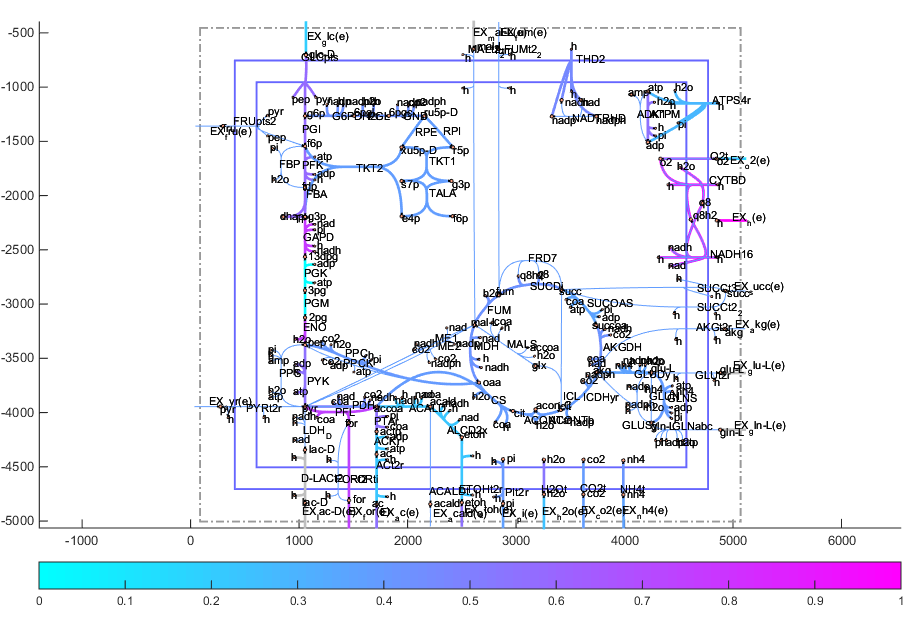
\includegraphics[scale=0.6]{grow_r_aer.png}}
    \caption{Состояние модели \textit{E.coli} с максимальной скоростью роста в аэробных условиях}
    \label{fig:gr_aer}
\end{figure}

\begin{figure}[H]
    \center{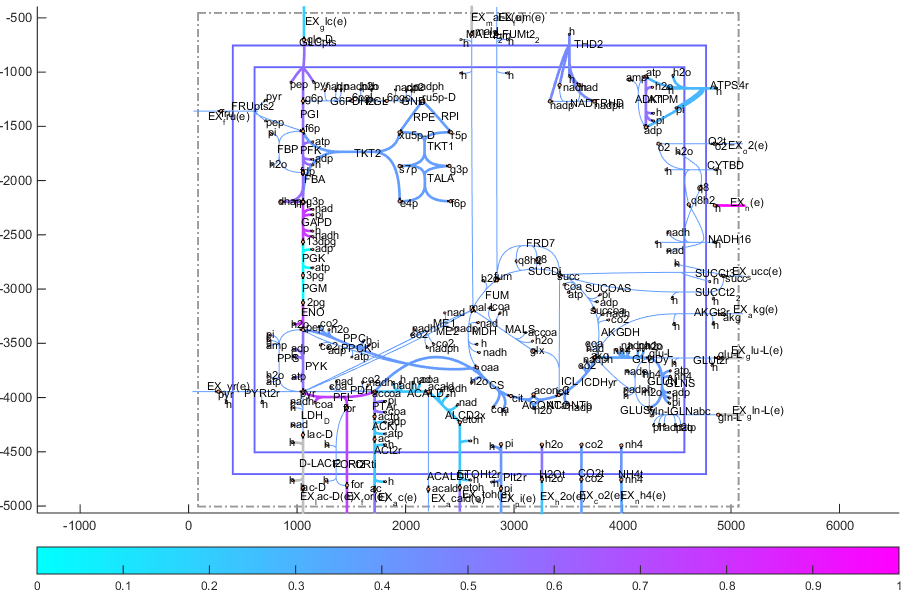
\includegraphics[scale=0.6]{grow_r_anaer.png}}
    \caption{Состояние модели \textit{E.coli} с максимальной скоростью роста в анаэробных условиях}
    \label{fig:gr_anaer}
\end{figure}

\subsection{Расчет темпов роста на альтернативных субстратах}

АМП также можно использовать для расчета скорости роста \textit{E.coli} на различных субстратах. Основная модель \textit{E.coli} содержит реакции обмена для 13 различных органических соединений, каждое из которых может использоваться в качестве единственного источника углерода в аэробных условиях. Например, чтобы смоделировать рост на сукцинате, нужно выполнить команды:
\begin{lstlisting}
    model = changeRxnBounds(model,'EX_glc(e)',0,'l');
    model = changeRxnBounds(model,'EX_succ(e)',-20,'l');
    FBAsolution = optimizeCbModel(model,'max');
\end{lstlisting}

Описание каждой субстрата содержится в \nameref{pr:2}. 

Чтобы смоделировать рост в анаэробных условиях с любым субстратом, нужно установить нижнюю границу кислородного обмена равной 0.

Результаты вычислений можно оформить в виде Таблицы \ref{t:1}:

\begin{table}[H]
\begin{tabular}{ |c|c|c| }
\hline
\multirow{}{}{Субстрат} & \multicolumn{2}{c|}{Скорость роста (1/ч)} \\ \cline{2-3} 
                          & Аэробные условия   & Анаэробные условия   \\ \hline
Acetate                   & 0,3893             & 0                    \\ \hline
Acetaldehyde              & 0,6073             & 0                    \\ \hline
2-oxoglutarate            & 1,0982             & 0                    \\ \hline
Ethanol                   & 0,6996             & 0                    \\ \hline
D-fructose                & 1,7906             & 0,5163               \\ \hline
Fumarate                  & 0,7865             & 0                    \\ \hline
D-glucose                 & 1,7906             & 0,5163               \\ \hline
L-glutamine               & 1,1636             & 0                    \\ \hline
L-glutamate               & 1,2425             & 0                    \\ \hline
D-lactate                 & 0,7403             & 0                    \\ \hline
L-malate                  & 0,7865             & 0                    \\ \hline
Pyruvate                  & 0,6221             & 0,0655               \\ \hline
Succinat                  & 0,8401             & 0                    \\ \hline
\end{tabular}
\caption{Максимальная скорость роста модели \textit{E.coli} на 13 различных органических субстратах, расчитанная АМП}
\label{t:1}
\end{table}

\subsection{Поиск альтернативных оптимальных решений}

Распределение потока, рассчитываемое АМП, часто не является уникальным. Во многих случаях биологическая система может достичь той же цели, используя альтернативные пути, поэтому возможны фенотипически различные альтернативные оптимальные решения. Метод, который использует АМП для определения альтернативных оптимальных решений, - это анализ изменчивости потока. Это метод, который определяет максимальные и минимальные возможные потоки через конкретную реакцию с целевым значением, которое должно быть близко или равным его оптимальному значению.


Например, для фермента ME1 последовательность вычислений выглядит следующим образом:

\begin{lstlisting}
    model = changeRxnBounds(model,'EX_glc(e)',0,'l');
    model = changeRxnBounds(model,'EX_succ(e)',-20,'l');
    FBAsolution = optimizeCbModel(model,'max');
    model = changeRxnBounds(model,'Biomass_Ecoli_core_w_GAM',FBAsolution.f,'b');
    model = changeObjective(model,'ME1');
    FBAsolutionMin = optimizeCbModel(model,'min');
    FBAsolutionMax = optimizeCbModel(model,'max');
\end{lstlisting}

Вычисления для различных ферментов представлены в Таблице \ref{t:2}:
\begin{table}[H]
\begin{tabular}{|c|c|c|}
\hline
Реакция                                  & Минимальный поток & Максимальный поток \\ \hline
FRD7 (fumarate reductase)                & 0                 & 972,77             \\ \hline
MDH (malate dehydrogenase)               & 13,56             & 20,06              \\ \hline
ME1 (malic enzyme (NAD))                 & 0                 & 6,49               \\ \hline
ME2 (malic enzyme (NADP))                & 7,17              & 13,67              \\ \hline
NADTRHD (NAD transhydrogenase)           & 0                 & 6,49               \\ \hline
PPCK (phosphoenolpyruvate carboxykinase) & 3,93              & 10,42              \\ \hline
PYK (pyruvate kinase)                    & 0                 & 6,49               \\ \hline
SUCDi (succinate dehydrogenase)          & 27,23             & 1000               \\ \hline
\end{tabular}
\caption{Различные реакции роста на сукцинате в аэробных условиях}
\label{t:2}
\end{table}

\subsection{Анализ устройчивости}

Другой метод, использующий АМП для анализа свойств сети, - это анализ устойчивости. В этом методе поток через одну реакцию варьируется, и оптимальное целевое значение рассчитывается как функция этого потока. Это показывает, насколько чувствительна цель к конкретной реакции. Есть много проницательных комбинаций реакции и цели, которые можно исследовать с помощью анализа устойчивости. Одним из примеров является изучение влияния поглощения питательных веществ на скорость роста. Для выполнения данного исследования нужно воспользоваться командами:
\begin{lstlisting}
    model = changeRxnBounds(model,'EX_o2(e)',-17,'b');
    growthRates = zeros(21,1);
    for i = 0:20
        model = changeRxnBounds(model,'EX_glc(e)',-i,'b');
        FBAsolution = optimizeCbModel(model,'max');
        growthRates(i+1) = FBAsolution.f;
    end
\end{lstlisting}

По результатам анализа устойчивости можно построить графики (Рис. \ref{fig:gr_r_1} и Рис. \ref{fig:gr_r_2}):

\begin{figure}[H]
    \center{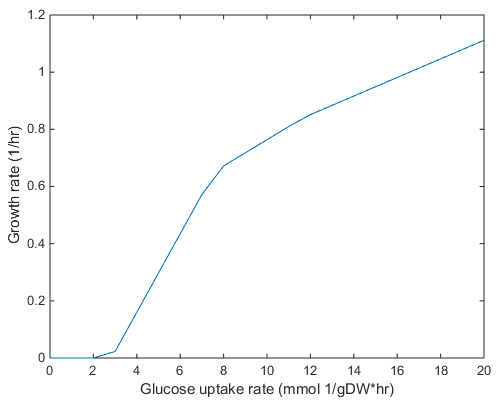
\includegraphics[scale=0.7]{r_a_1.png}}
    \caption{Анализ устойчивости для максимальной скорости роста при изменении скорости поглощения глюкозы при фиксированном поглощении кислорода на уровне 17 ммоль/gDW $\cdot$ час}
    \label{fig:gr_r_1}
\end{figure}

\begin{figure}[H]
    \center{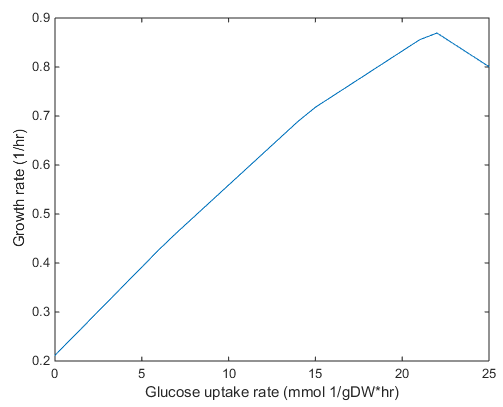
\includegraphics[scale=0.7]{r_a_2.png}}
    \caption{Анализ устойчивости для максимальной скорости роста при изменении скорости поглощения кислорода при фиксированном поглощении кислорода на уровне 10 ммоль/gDW $\cdot$ час}
    \label{fig:gr_r_2}
\end{figure}

\subsection{Исследование фенотипических фазовых плоскостей}

При выполнении анализа устойчивости изменяется один параметр и вычисляется состояние сети. Также возможно изменять два параметра одновременно и отображать результаты в виде фенотипической фазовой плоскости. Например, можно рассчитать фенотипическую фазовую плоскость для максимального роста при изменении скорости поглощения глюкозы и кислорода. Для этого необходимо выполнить команды:
\begin{lstlisting}
    growthRates = zeros(21);
    for i = 0:20
        for j = 0:20
            model = changeRxnBounds(model,'EX_glc(e)',-i,'b');
            model = changeRxnBounds(model,'EX_o2(e)',-j,'b');
            FBAsolution = optimizeCbModel(model,'max');
            growthRates(i+1,j+1) = FBAsolution.f;
        end
    end
\end{lstlisting}

Результат можно представить в виде 2D и 3D графика (Рис. \ref{fig:ph_ph_2}).

\begin{figure}[H]
    \center{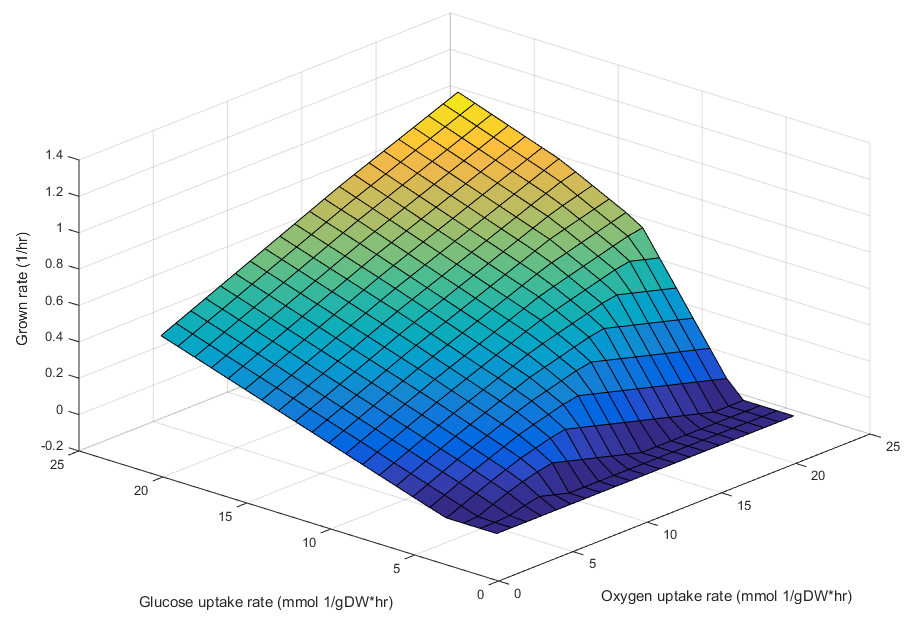
\includegraphics[scale=0.6]{phen_ph_pl_analys.png}}
    \label{fig:ph_ph}
\end{figure}

\begin{figure}[H]
    \center{\includegraphics[scale=0.6]{phen_ph_2.png}}
    \caption{Фенотипические фазовые плоскости для роста с различной скоростью поглощения глюкозы и кислорода.}
    \label{fig:ph_ph_2}
\end{figure}

\subsection{Моделирование нокаутов генов}

Подобно тому, как рост в различных средах можно моделировать с помощью АМП, нокауты генов также можно моделировать, изменяя границы реакции. Чтобы смоделировать нокаут любого гена, можно просто ограничить связанную с ним реакцию или реакции, чтобы они не переносили поток. Это можно сделать с помощью функций:
\begin{lstlisting}
    [grRatio,grRateKO,grRateWT] = doubleGeneDeletion(model);
    imagesc(grRatio)
    xlabel('gene knockout 1')
    ylabel('gene knockout 2')
\end{lstlisting}

В результате получаем (Рис. \ref{fig:s_g_k}):
\begin{figure}[H]
    \center{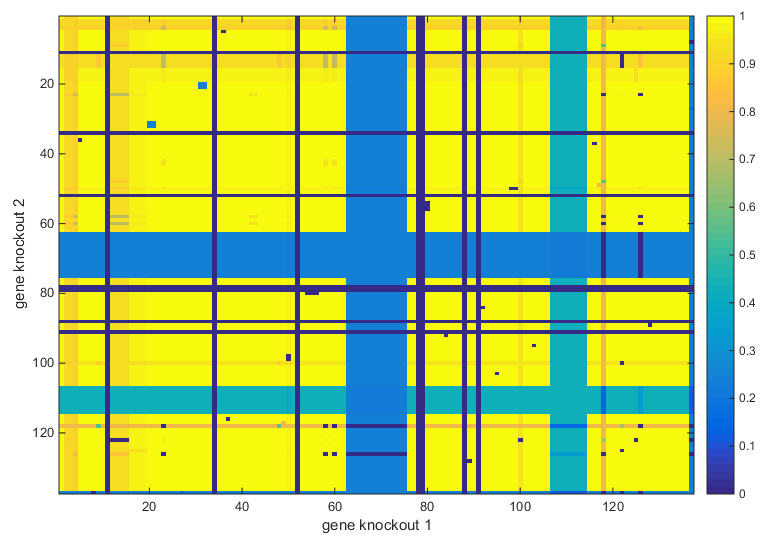
\includegraphics[scale=0.6]{sim_g_knoc.png}}
    \caption{Скрининг нокаута гена по глюкозе в аэробных условиях}
    \label{fig:s_g_k}
\end{figure}

\subsection{Нокаут каких несущественных генов оказывает наибольшее влияние на гибкость сети?}

Также можно исследовать следующий вопрос: каковы последствия для сети удаления несущественного гена? Для начала нужно удалить сетевые гены по отдельности (исследование делеции одного гена), а затем выполнить АМП на штаммах с несущественными делециями генов. Во многих случаях можно ожидать, что удаление гена имеет лишь незначительные последствия для сети, особенно если удаление не влияет на максимальную скорость роста. Однако в некоторых случаях удаление может снизить общую гибкость сети или, возможно, даже увеличить диапазон потока за счет определенных реакций. Для данного исследования нужно выполнить следующую последовательность действий:
\begin{lstlisting}
    [minFluxAll(:,1),maxFluxAll(:,1)] = fluxVariability(model);
    genes=model.genes([2,14,16,23,42,48]);
    for i = 1 : length(genes)
        [modelDel] = deleteModelGenes(model,genes{i});
        [minFluxAll(:,i+1),maxFluxAll(:,i+1)] =
        fluxVariability(modelDel);
    end
    fluxSpan = abs(maxFluxAll - minFluxAll);
    for i = 1 : size(fluxSpan,2)
        fluxSpanRelative(:,i) = fluxSpan(:,i)./fluxSpan(:,1);
    end
    for i =2:7
        subplot(2,3,i-1)
        hist(fluxSpanRelative(:,i),20);
        title(genes{i-1});
    end
\end{lstlisting}

В результате получаем гистограммы (Рис. \ref{fig:n_e}):
\begin{figure}[H]
    \center{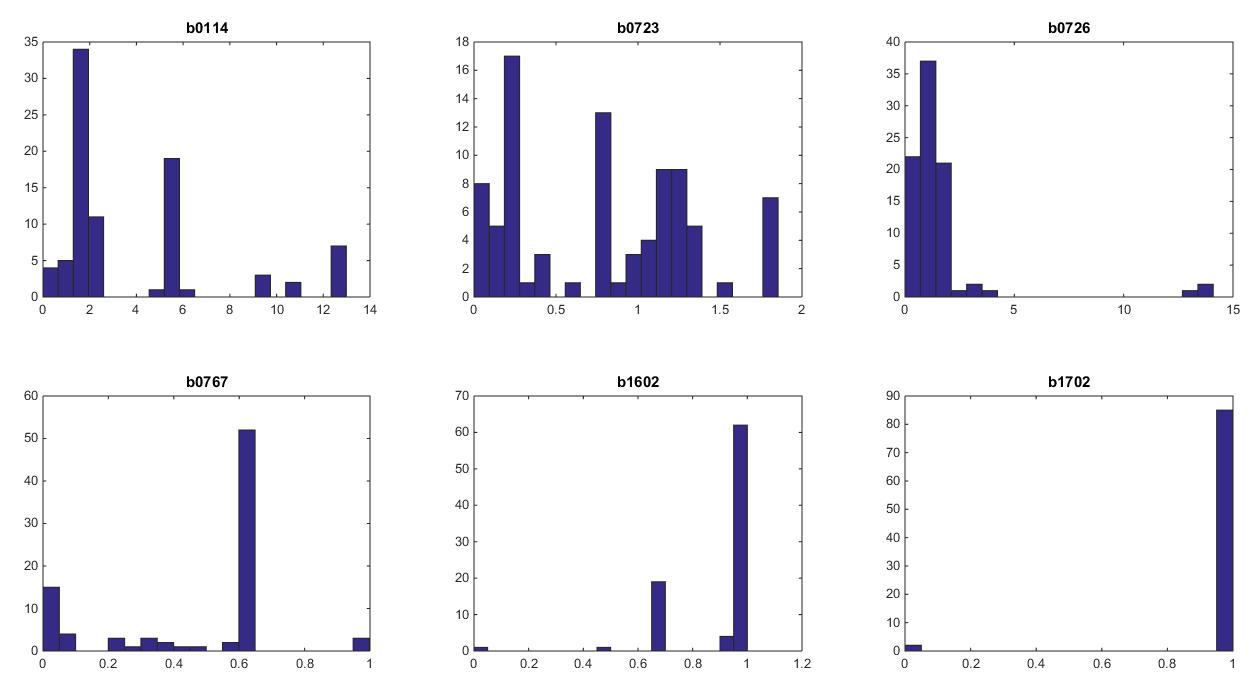
\includegraphics[scale=0.5]{n_e_g_k.png}}
    \caption{Гистограммы относительных интервалов потоков для 6 мутантов с нокаутом генов}
    \label{fig:n_e}
\end{figure}

\subsection{Исследование топологических особенностей матрицы $S$}

\subsubsection{Визуализация матрицы $S$}

Матрица $S$ базовой модели \textit{E.coli} может быть визуализирована с помощью команды |spy|. Эта команда представит все ненулевые записи в S точкой
\begin{lstlisting}
    spy(model.S);
\end{lstlisting}

В результате получаем следующее представление (Рис. \ref{fig:S})
\begin{figure}[H]
    \center{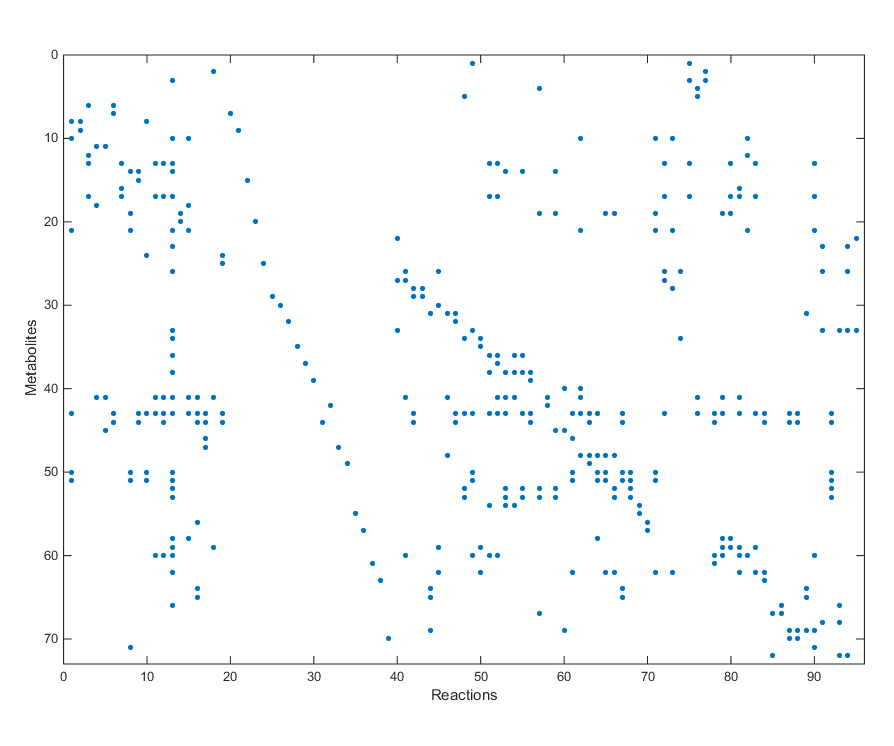
\includegraphics[scale=0.5]{matrix_S.png}}
    \caption{Стехиометрическая матрица $S$ (размера 72 $\times$ 95) модели \textit{E.coli}}
    \label{fig:S}
\end{figure}

\subsubsection{Определение количества реакций, в которых происходят метаболиты}

Матрица S может быть преобразована в двоичную матрицу путем замены всех ненулевых элементов в S на 1. Затем все единицы в каждой строке можно суммировать, чтобы определить количество реакций, в которых происходит метаболит. Для этого нужно выполнить последоательность команд
\begin{lstlisting}
    Sbin = zeros(size(model.S));
    Sbin(find(model.S))=1;
    for i = 1 : length(model.mets)
        metConnectivity(i,1) = sum(Sbin(i,:));
    end
    loglog(sort(metConnectivity,'descend'),'*')
    xlabel('metabolite number (rank ordered) - log scale’);
    ylabel('number of reactions - log scale')
\end{lstlisting}

В результате получаем график (Рис. \ref{fig:det_numb}):
\begin{figure}[H]
    \center{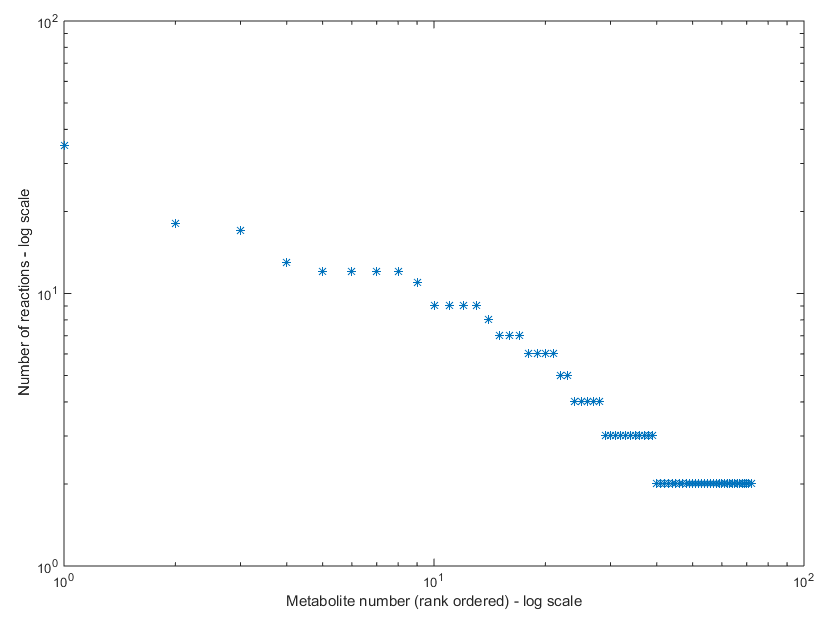
\includegraphics[scale=0.5]{det_numb_reac_metab_occur.png}}
    \caption{Связность основных метаболитов \textit{E.coli}}
    \label{fig:det_numb}
\end{figure}

\newpage
\section*{Заключение}
\addcontentsline{toc}{section}{Заключение}

В результате исследований можно сказать, что COOBRA Toolbox - это удобный инструмент для работы с метаболическими сетями. С помощью данного пакета можно делать и визуализацию данных, и их анализ. 

\newpage
\addcontentsline{toc}{section}{Список используемых источников}
\begin{thebibliography}{}
    \bibitem{litlink3} Orth, J. D., Thiele, I. & Palsson, B. Ø. What is flux balance analysis? Nature Biotechnology 28, 245–248 (2010).
    \bibitem{litlink1} \url{https://opencobra.github.io/cobratoolbox/stable/}
    \bibitem{litlink2} \url{https://systemsbiology.ucsd.edu/Downloads/EcoliCore}
\end{thebibliography}

\newpage
\section*{Приложение 1} \label{pr}
\addcontentsline{toc}{section}{Приложение 1}

Код программы и данные расположены в репозитории GitHub по ссылке: \url{https://github.com/Drozdova-Daria/Practice_Cobra}

\newpage
\section*{Приложение 2} \label{pr:2}
\addcontentsline{toc}{section}{Приложение 2}

Функции для вычисления скорости роста на различных субстратах

\begin{table}[H]
\begin{tabular}{ |c|c| }
\hline
Название субстрата & Функция для вычиления \\ \hline
Acetate            & | EX_ac(e) |          \\ \hline
Acetaldehyde       & | EX_acald(e) |       \\ \hline
2-oxoglutarate     & | EX_akg(e) |         \\ \hline
Ethanol            & | EX_etoh(e) |        \\ \hline
D-fructose         & | EX_fru(e) |         \\ \hline
Fumarate           & | EX_fum(e) |         \\ \hline
D-glucose          & | EX_glc(e) |         \\ \hline
L-glutamine        & | EX_gln_L(e) |       \\ \hline
L-glutamate        & | EX_glu_L(e) |       \\ \hline
D-lactate          & | EX_lac_D(e) |       \\ \hline
L-malate           & | EX_mal_L(e) |       \\ \hline
Pyruvate           & | EX_pyr(e) |         \\ \hline
Succinate          & | EX_succ(e) |        \\ \hline
\end{tabular}
\end{table}

\end{document} 
